\documentclass[10pt,twocolumn]{article}

% use the oxycomps style file
\usepackage{oxycomps}
\usepackage{float}
\usepackage{biblatex}
\addbibresource{references.bib}
\usepackage{enumitem}

\pdfinfo{
    /Title (Resolving Economic Puzzles with Psychology through Simulation)
    /Author (Oliver Wilkins)
}

% set the title and author information
\title{Resolving Economic Puzzles with Psychology through Simulation}
\author{Oliver Wilkins}
\affiliation{Occidental College}
\email{wilkins@oxy.edu}

\begin{document}

\maketitle

\section{Problem Context}
The standard economic theory which has dominated the field over the past century is once which derived from a realization in the early 1900s that consumer choice theory “did not require knowledge about the psychic intensity of individual’s preferences, but only that preferences were consistently ordered.”\cite{lehr} This realization allowed economists to formalize theory which did not explicitly consider the psychological factors behind people’s decisions. While this standard theory was a powerful and technically convenient way to make sense of much of human decision-making and its aggregate effects, there were a number of ‘anomalies’ observed in real world behavior. An ‘anomaly’ in this context is a behavior which under standard theory is either impossible to predict or requires using values for certain economic parameters which are outside the generally accepted range within the literature. The field of behavioral economics arose within the past few decades in an attempt to explain these various anomalies by explicitly integrating aspects of human psychology into existing economic models so as to be able to predict behaviors which are ‘irrational’ as defined by standard economic theory.

One area in which several of these anomalies exist is the stock market. In particular, economists have generally identified three features of people’s interaction with the stock market which are puzzling under a standard framework. These features are:
\begin{enumerate}
    \item The equity premium puzzle
    \item The existence of asset price bubbles 
    \item Underinvestment
\end{enumerate}
 The equity premium puzzle is defined as the empirical observation that the equity premium, or the excess return of stocks relative to bonds, implies a much higher level of risk aversion than is implied by data from other contexts involving decision-making under uncertainty. Asset price bubbles are defined as periods in which prices of an asset or class of assets exceed their fundamental value. They constitute a puzzle because the efficient market hypothesis suggests that any deviation of price from fundamental value would be quickly undone by market forces, yet empirically bubbles can exist for relatively long time periods. Underinvestment is defined as the empirical observation that people do not invest in the stock market as much as would be optimal for them to maximize their lifetime utility, or well-being, even when accounting for the fact that people discount the utility of their future selves relative to their present selves.

The general structure of my project is to simulate the stock market in various ways to see if it is possible to predict the anomalies introduced above by including concepts from behavioral economics within the models. The value of this project is in attempting to support the validity of the behavioral economic methodology within the context of the stock market. It is not intended to generate empirically accurate results or to contribute to the literature on estimating the true value of any of the parameters I use. Rather, a successful version of my work would be one which persuades those reading it that the behavioral economic concepts included are ones which capture true aspects of human nature that should be included in economic research going forwards so as to better model the world and therefore create better public policy. It is also important to note that the behavioral changes I make to standard theory are not novel, i.e. in each case there already exists work suggesting that the change in question is a plausible explanation for the given puzzle. Rather, I am either extending existing work or taking a slightly different approach to the same question.

\section{Technical Background}
In this section, I will discuss the technical background necessary to understand the justification for setting up each of the three simulations in the way I do. For each, I will first discuss the relevant standard framework under which the behavior in question constitutes an anomaly. I will then examine one or two concepts from behavioral economics which theoretically help to explain the anomaly. After each model has been covered, I will discuss the technique of simulation in a general sense.  

\subsection{Equity Premium Puzzle}
The equity premium puzzle is one of the most famous in economics. That returns on stocks are so much higher than on bonds constitutes a puzzle because this increased return should increase demand for stocks relative to bonds, lowering the difference between their returns. This is not to say that the existence of an equity premium is an anomaly under standard economics. Because stocks are riskier than bonds and people are assumed to be risk averse, defined as a preference for certain outcomes over uncertain outcomes with the same expected value, there must exist a positive equity premium. However, the magnitude of the premium should be reflective of the extent to which people are risk averse, and the historical magnitude of the premium implies a level of risk aversion far higher than anything within the generally accepted range within the literature. This will be explored further in the prior work section. 

The standard models predicts that people will make their decision of whether to enter the stock market at a given equity premium based on the expected utility of doing so compared to expected utility of purchasing bonds. Expected utility is the weighted average of the utilities of the various possible outcomes, weighted by the likelihood of those outcomes. Risk aversion comes into play because the utility function used to evaluate outcomes is not simply equal to their net gain or loss. Rather, it is some concave function over their wealth as a result of the net outcome. The specific function used in this project is constant relative risk aversion, as is common within the literature. shown below: 
\begin{figure}[H]
    \centering
    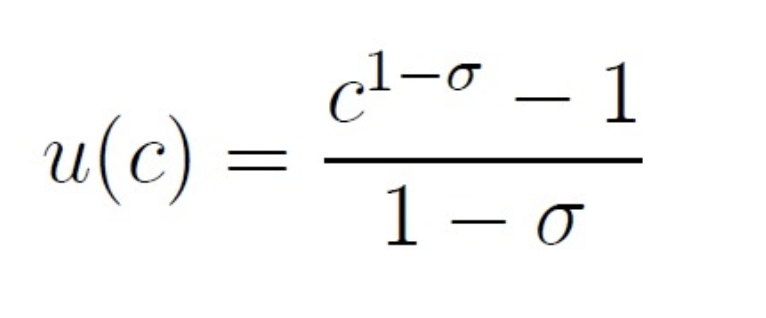
\includegraphics[width=0.5\linewidth]{images/crra.png}
\end{figure}
\noindent where $\sigma$ represents the degree of risk aversion. The concavity of the function implies risk aversion, because an increase in wealth will increase utility by a smaller amount that a decrease of the same size decreases it. Crucially, this model assumes that people pre-determine for how long they would hold a stock if they were to buy it and only consider the expected utility as calculated at the end of that period, with no consideration for its intervening fluctuations. 

In an attempt to explain the equity premium, my simulation will introduce two concepts from behavioral economics. They are loss aversion and bracketing. Loss aversion is the phenomena that people tend to perceive the pain of losing something to be about twice as large in magnitude to the positive emotion associated with gaining something of equivalent value. Loss aversion can help explain the equity premium because people are overweighting potential losses relative to potential gains, causing them to demand higher returns in order to take on risk. Bracketing, in this context, is the idea that people pay attention to the fluctuations of the market rather than to their net returns once they have sold the stock. This is relevant because the chance of having a loss in any given day, month, year, etc. is quite high, whereas the chance of having a net loss after tens of years is approximately zero. If people are also loss averse over the returns of these individual periods, it becomes clear how the returns they demand are much higher than those predicted by risk aversion alone.

\subsection{Bubbles}
Underlying the efficient market hypothesis is the assumption that people form their beliefs about the fundamental value of a stock based on all publicly available information, and then accurately update that belief when they receive new information, whether that be in the form of price changes to the stock or new information about the company in question. To be accurate, a person must update their belief in accordance with Bayes rule, written out below:
\begin{figure}[H]
    \centering
    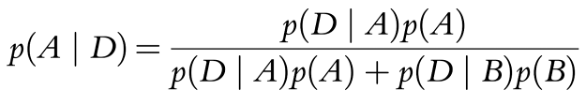
\includegraphics[width=1\linewidth]{images/EMH1.png}
\end{figure}

\noindent where A and B are the possible states of the world. Given some new information D, the above formula allows a person to accurately update their belief about the probability that A is the true state of the world. Under the assumption of universal Bayesian belief updating the existence of bubbles is not possible. A possible explanation for these observations comes from the behavioral economics literature on non-standard belief updating, in particular the existence of extrapolative beliefs. Extrapolative beliefs are the result of an incorrect belief in the law of small numbers, which is the idea that a small sample will necessarily ‘look like’ the larger population from which it is drawn. Someone with extrapolative beliefs who sees that a stock has positive returns for multiple consecutive periods will therefore believe with too much confidence that the fundamental value of the stock is high. A portion of the population having such beliefs could plausibly explain the existence of bubbles.

\subsection{Underinvestment}
The standard framework for modeling a person’s lifetime savings and investment decisions is an extrapolation of the discounted utility model called the life-cycle model, formalized by Modigliani and Brumberg in 1954.\cite{modigliani} Under this model, people have a utility function over their lifetime consumption which looks different in each period, where period can be defined by any unit of time. In this context, a utility function is a function which translates a series of consumption levels into an overall quantification of well-being. It looks different in each period because people discount future periods relative to how far they are from the current one, typically modeled as being in an exponential fashion. This function, from the perspective of period 0, takes the following form:
\begin{figure}[h]
    \centering
    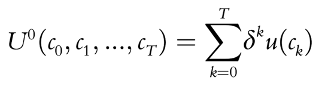
\includegraphics[width=0.8\linewidth]{images/Underinvestment1.png}
\end{figure}

\noindent where $0 < \delta < 1$, $c_i$ is consumption in the ith period, there are t more periods left in a person's life, and $u(c_k)$ is some function which transforms consumption in period k to utility. These consumption values must be bounded by the income one will have over the course of their life, which can be expressed mathematically as follows:
\begin{figure}[h]
    \centering
    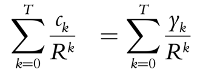
\includegraphics[width=0.5\linewidth]{images/underinvestment2.png}
\end{figure}

\noindent where $R^k$ is the gross per-period interest rate, $C_k$ is the consumption in period k, and $Y_k$ is the income in period k. Under this model, people will make their savings decisions by maximizing the utility function subject to the budget constraint, expressed mathematically below:
\begin{figure}[h]
    \centering
    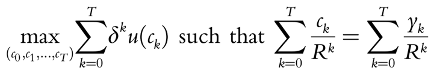
\includegraphics[width=1\linewidth]{images/underinvestment3.png}
\end{figure}

For the purpose of simplicity, the above model is one in which there is certainty about lifespan, future earnings, and interest rates. While in the real world such certainty obviously does not exist, its inclusion does not limit the model's ability to estimate the effects we are interested in.

The key feature of the above model, for our purposes, is that people are necessarily time consistent. Time consistency means that if they plan in one period to save a certain amount in a subsequent period, they will actually end up saving their planned amount when that subsequent period arrives. However, empirical evidence (and intuition) does not support the model’s prediction of time consistency, as will be examined in the prior work section. In an attempt to rectify this disparity between the model and reality, my simulation includes the concept of present bias. Present bias is the idea that people discount any period which is in the future by some constant amount in addition to the standard exponential discounting. This constant discounting is meant to account for the fact that people only ever exist in the present, and therefore overvalue it relative to anytime in the future, regardless of how far. Present bias modeled in this way allows for time-inconsistent preferences.  


\subsection{Agent-Based Simulation}
Simulation is a technique which seeks to mimic a real-world process for the purpose of being able to manipulate parameters and see the effect of doing so. While a simulation relies upon a model of the world such as those previously discussed, it is more dynamic in that it has the advantage of being able to incorporate randomness over time and to apply the model to different agents who may have different characteristics and who can interact with each other. This project sometimes uses agent-based simulation, a type of simulation which focuses on the characteristics and decisions of individuals and how the aggregation of those decisions creates the system we observe. In the words of Eric Bonabeau, a leader in the fields of complex systems and human decision-making, “ABM is a mindset more than a technology. The ABM mindset consists of describing a system from the perspective of its constituent units… [which] enables one to deal with more complex individual behavior, including learning and adaptation.”\cite{bonabeau}

\section{Prior Work}
This section will explore literature related to each of the three simulations, with two goals in doing so. The first is to examine past work that has been done to explain the anomaly and discuss how my project will complement this existing work. The second is to identify the sources from which relevant data and empirical estimates of parameters will be sourced, for the simulations for which this is needed.



\subsection{Equity Premium Puzzle}
The equity premium puzzle is a famous question within economics, and much has been written on its possible causes. In 1997, the influential behavioral economist Richard Thaler wrote a paper with colleague Jeremy Siegal in which they survey possible explanations and conclude that it is very difficult to explain the puzzle without some sort of irrationality of the type behavioral economics is focused on.\cite{thaler}  In 2007, Barberis and Huang were among the first to formalize the bracketing and loss aversion explanation of the equity premium puzzle, finding that the approach was promising and merited further research.\cite{BarberisEPP} My work complements theirs by using a similar approach with newer data and a different time horizon, as well as investigating the effects of variable bracket sizes as opposed to only loss aversion values. The series of lotteries which I will use in order to model the stock market for the purpose of investigating the equity premium puzzle is a common way of modeling it within the behavioral economics literature. The sources of the data I use to construct my model are listed below:
\begin{enumerate}
    \item historical equity premiums\cite{equitypremiums}
    \item utility function over wealth\cite{utilitywealth}
    \item empirical estimation of loss aversion coefficient\cite{lossaversion}
\end{enumerate}

\subsection{Bubbles}
Violations of the efficient market hypothesis have been pointed out for nearly as long as the hypothesis itself has been around. References to some of many papers responsible for documenting specific violations, i.e. bubble instances, are linked.\cite{MedTermMomentum}\cite{LongTermReversal}\cite{volatility}\cite{bubbles} The idea of using extrapolative beliefs to formally account for the existence of bubbles with a simulation-based approach is credited to Barberis et. al..\cite{BarberisEtAl} Their work established extrapolative beliefs as a plausible explanation for the existence of bubbles, and estimated the proportion of agents within the model who must hold such beliefs in order for a bubble of a given size to be generated. My work extends this by estimating the difference in bubble size between models in which the non-extrapolative agents are aware of extrapolative ones and models in which they are not. 


\subsection{Underinvestment}
Much of the literature around low savings and investment rates focuses on structural barriers to these behaviors, such as increasing cost of living relative to wages and the disappearance of pensions. Still, the fact remains that people consistently report not saving as much for their retirement as they would like to be given their circumstances. A recent example of this comes from the TransAmerica center for Retirement Research’s annual report\cite{transamerica}, finding that 73\% of those 50 and older wished they had saved more on a consistent basis. Additionally, the report finds that nearly half of retirees decrease their consumption in retirement. Both of these figures contradict the standard model and point towards the need for explanations beyond structural challenges. Among the research in this area, present bias is a leading explanation. Goda et. al\cite{goda} find that an individual’s score on a questionnaire designed to detect present bias is correlated with their level of retirement savings. There has been work in integrating present bias into simulations of the life-cycle model, such as Peter Maxted’s work in estimating the welfare costs of present bias in the context of savings decisions.\cite{maxted} 

Below is a list of the areas in which data is needed and a link to the reference for the location from which the data will be obtained:
\begin{enumerate}
    \item historical return on savings\cite{returns}
    \item life expectancy data\cite{death}
    \item generally accepted range for the magnitude of present bias\cite{presentbias}
\end{enumerate}

\section{Methods}
This section will discuss the setup of each of the three simulations. It will first include how the standard model will be set up and calibrated, and then how the relevant behavioral concept(s) will be included and calibrated, where relevant. In every case where the value of a parameter is drawn from some distribution, the distribution is determined by empirical work discussed in the above section.

The general process of converting economic theory into simulations starts with identifying the decision that agents are making in a given situation, e.g. wether to invest in stocks or in bonds in the equity premium puzzle example. I then set up the simulation such that the aggregate result of that decision takes the form of something which can be compared to empirical data, e.g. the equity premium. From there my focus turns to manipulating the agent's actual decision-making process, which is the focus of this project. I first have the agent make their decision according to the rules of standard economics, i.e. as though they were perfectly rational. I compare the results of the simulation under this decision-making processes to the results when I break the assumption of perfect rationality in ways consistent with the psycology literature. 



\subsection{Equity Premium Puzzle}
\subsubsection{Standard Setup and Calibration}
To investigate the equity premium puzzle, I simulate only one agent, meant to be representative of a typical investor. I restrict their decision set to two choices: invest \$100 in bonds for 10 years, or invest \$100 in the S\&P 500 index for 10 years. If the agent chooses bonds, they get a guaranteed return, calculated by taking the historical average of US 10 year treasuries. Their expected utility from making this choice is calculated simply by plugging that guaranteed end result into their utility function. The model uses a constant relative risk aversion utility function, as is common within the literature. 

To calculate the expected utility of choosing to invest in stocks, I first collect historical data on monthly returns of the S\&P 500 and create a distribution of these returns. I then model the choice of investing in stocks as drawing randomly from this distribution 120 times, i.e. every month for 10 years. After each draw the agent's money is multiplied by 1 + the return. At the end of 10 years, the end result is plugged into the utility function. This process is repeated 10,000 times, with results averaged. I chose this approach because the computational complexity of calculating every possible combination of returns was too high to be feasible. Once all 10,000 trials are averaged, that average is compared to the utility of choosing to invest in bonds. Whichever choice results in a higher expected utility is the one the agent chooses. 

To prove that the results of this simulation constitute a puzzle, I manipulate the coefficient of risk aversion within the utility function such that the agent is indifferent between the two options, i.e. their expected utilities are the same. The point of indifference matters because, if we assume the model is correct, the equity premium will be such that agent is indifferent, as per the market mechanism. However, for this to be the case within the simulation the coefficient of risk aversion must approximately equal 8, which is outside the typical range within the literature. The model must therefore be flawed. 

\subsubsection{Introduction of Behavioral Factors}
To improve the model so that it can predict the empirically observed equity premium without relying on unrealistic values of parameters, I introduce bracketing and loss aversion. Computationally, this entails a change to the way that expected utility is calculated if the agent chooses to invest in stocks. Rather than plugging the net result after 10 years into the utility function, the result at the end of each period equal in size to the bracketing value gets plugged in. The agent's reference point is reset each time this is done to whatever their current wealth is. Loss aversion is modeled in the following way: each time utility is calculated, if the net return over that period is negative, the loss is multiplied by the loss aversion coefficient before being plugged into the function. The risk aversion parameter is no longer allowed to vary, but instead is fixed at its median estimated value of 2. 

I manipulate both loss aversion and bracketing values within reasonable ranges and compute the utility differential for each combination. Combinations which result in indifference between buying stocks and buying bonds are possible explanations of the equity premium puzzle. 

\subsection{Violation of Efficient Market Hypothesis}
\subsubsection{Standard Setup}
For simplicity, this simulation will be over a singe asset. There will be 100 agents who are each assigned a valuation randomly from a normal distribution, representing their belief as to the fundamental value of the stock. Agents are not aware of where they fall within this distribution. Each agent is given an endowment of the stock and of cash.

The simulation lasts for 50 periods. In each period the fundamental value of the asset increases by some amount. The agents update their belief accordingly, but the width of the distribution of their beliefs does not change. In each period the agents are free to trade with one another, assuming they have either the shares or the cash to do so. Their trading decision is simple: buy if their valuation is higher than the market price and sell if it is not. The market price in a given period is a function of the previous market price and the ratio of agents who wish to sell vs buy. 

The increase in fundamental value is constant for the first 10 periods. For the next 3 it increases at a significantly quicker pace before returning to the initial one, meant to model some good news about the underlying asset. The expectation is that because all of the agents are rational, i.e. operate in accordance with Bayes rule, the good news shouldn't cause any deviation of price from fundamental value. Because empirically good news about an asset can trigger a bubble, there is something missing in this model.

\subsubsection{Introduction of Behavioral Factors}
In this stage, a portion of the 100 agents are assigned to have extrapolative beliefs, meaning they interpret the price change in response to the news relating to the value of the stock as more indicative of a change in fundamental value than it actually is. I test the effect of varying this proportion on the resulting bubble size, as calculated by taking the sum of the differences between fundamental value and price for the periods in which price exceeds fundamental value. 

I  also test the effect of rational agents being aware of the existence of extrapolative agents on bubble size for given proportions of extrapolative agents. I model this by changing the rational agent's price expectations to have two components: their belief of fundamental value weighted by 1 - the proportion of extrapolative agents plus the recent price momentum weighted by the proportion of extrapolative agents. 

\subsection{Underinvestment}
\subsubsection{Standard Setup and Calibration}
The simulation is set up as a series of 64 periods, each representing a single year. A single agent is created with a starting age of 22, starting wealth of \$10,000, and starting salary of \$50,000. They have a utility function over life-cycle consumption as described in the technical background section, with a discount factor of 0.95. Retirement age is fixed at 65, and death age is fixed at 85. For simplicity, agents receive the same income in every period up to retirement. In retirement, they receive a social security payment of \$22,000, which is a typical value for people in that income range. In each period, the agent must make a choice which optimizes their expected lifetime utility from the perspective of the current period.
Ideally, the way the way the agent would calculate their optimal consumption in any given period would be via backwards induction. This means they would start in the final period and consider what they would do in any given situation. They would then consider what they would do in the second to last period in any given situation, factoring in how their future self in the final period will respond to their choice. This process would continue until the period in which the choice is being made. However, I was simply unable to implement this approach given my programming ability and time constraints. Instead, I took advantage of the fact that the solution to the optimization problem of lifetime consumption choices tends towards being smooth consumption, i.e. the same in every period. I therefore modeled the choice of consumption by discretizing both the set of feasible options for the current period and for all future periods, assuming that the agent intended to have smooth consumption in all future periods but did not necessarily have to in the current one. I then tested each combination of these values to see which one gave the highest lifetime utility value. The current consumption value for that combination was chosen as the agent's choice, and the simulation moved into the next period. I first run the simulation with agents who are not present biased. 
 
\subsubsection{Introduction of Behavioral Factors}
In the second run of the simulation, I introduce present bias into the agent's utility calculation. Present bias is modeled computationally as a multiplier applied to the utility of every period which is not the present. It is separate from standard exponential discounting, and does not scale with time. I use the mean estimate within the literature of 0.7.

\section{Evaluation Metrics}
The metric for evaluating the success of the simulations is wether the inclusion of behavioral economic concepts resolves the puzzle which exists without them. What this entails for each individual simulation has been described in the previous section. In this section, I will argue that successful simulations as defined by this metric constitute an effective argument in favor of the validity of behavioral economics concepts as true aspects of human nature whose inclusion improves economic frameworks. While the models upon which the simulations depend are vast oversimplifications given the complexities of the world, they are still effective at telling an intuitive and logically valid story about people’s motivations within a certain context. Given that both the models with and without behavioral considerations suffer from this same limitation, if the models with behavioral considerations do a better job of replicating reality the behavioral factors must be true aspects of human nature. Beyond supporting the validity of the ideas of behavioral economics, this project also supports their increased inclusion in empirical research going forwards, as it adds to existing work in which they are successfully integrated with existing models and empirical data. See the 2023 report by the National Academies of Sciences, Engineering, and Medicine on the potential for behavioral economics to improve policy-making.\cite{report23} 

\section{Results and Discussion}
In this section I will walk through my results, explaining how to interpret them and how they fit with existing literature. I will then discuss the ways in which the limitations of my methods should inform caution in using their results to make claims about the world.  

\subsection{Equity Premium Puzzle}
I start by holding loss aversion constant at its mean estimate of 2 and allowing the bracket size to vary. The following graph shows the effect of each bracket size value on the utility differential between buying stocks and buying bonds. A negative differential means that a person who thinks according to the given bracket size would prefer to buy bonds at the empirically observed equity premium, whereas a positive one means they would prefer to buy stocks. 
\begin{figure}[H]
    \centering
    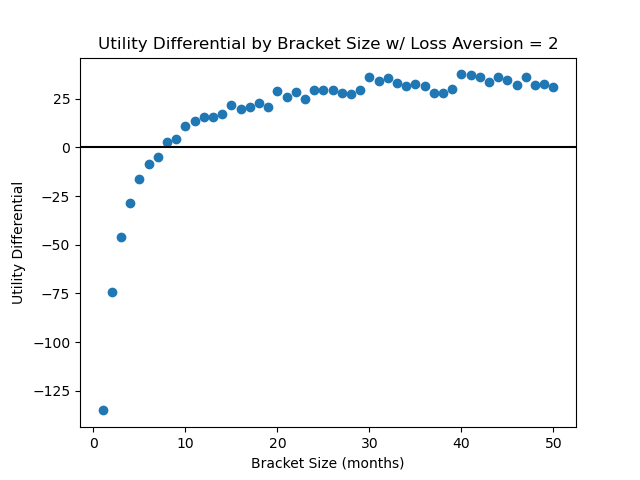
\includegraphics[width=0.8\linewidth]{images/EPP1.png}
    \label{fig:enter-label}
\end{figure}

Reading off the graph gives a point of indifference at a bracket size of approximately 10 months. This means that if every market participant had a loss aversion coefficient of 2 and a bracket value of 10 months, the equity premium puzzle would be solved.

I then allow loss aversion to vary as well. Each column in the graph below can be thought of as a version of the previous graph with a different loss aversion value. The utility differential is now represented with colors to allow for three dimensions to the graph. Purple areas represent combinations of loss aversion and bracket size for which people would prefer to buy bonds at the empirically observed equity premium, whereas green areas indicate they would rather buy stocks. The white sections indicate combinations for which the person is indifferent, i.e. the solution space to the equity premium puzzle.

\begin{figure}[H]
    \centering
    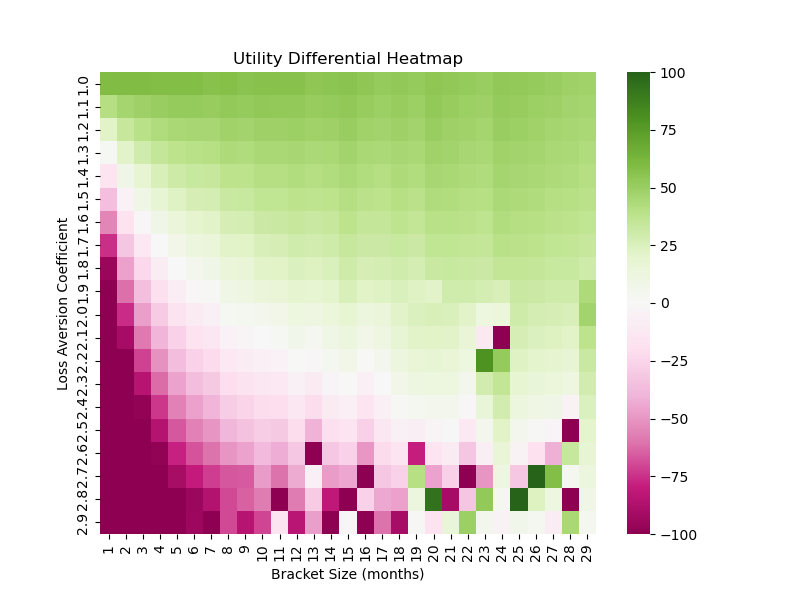
\includegraphics[width=0.8\linewidth]{images/EPP2.png}
    \label{fig:enter-label}
\end{figure}

The solution space is downward sloping and appears to be slightly curved, i.e. as bracket size increases the loss aversion coefficient required to create indifference also increases, but at a decreasing rate. The direction of the trend makes intuitive sense. For utility to be constant, as people are more loss averse they must think in longer time horizons to compensate for the increased utility penalty of loss with a decreased likelihood of experiencing it. The apparent curvature does not have as easy of an intuitive explanation, and may be more the result of fuzzy data in the bottom right quadrant of the graph than any real relationship between the variables. This fuzziness is the result of higher variability when both bracket size and loss aversion are high. In this situation periods of loss are more consequential but also more rare, meaning there will be higher variance in utility differential across random trials. Given the computing power I had access to I was unable to perform sufficient trials to smooth out this section. 

This work contributes to the literature by confirming findings by others who have investigated this topic but with different methods, increasing the robustness of the result. See Barberis\cite{BarberisEPP} and Dimmock and Kouwenberg\cite{dimmock} for examples of similar findings with different methods. I am not aware of any other work that estimates a 2-dimensional solution space in the way I do. 

The main drawback of my approach is that it does not account for variations in time horizon. This means that while my results provide a reasonable approximation of possible solutions to the equity premium puzzle, they are limited in that the assumption everyone invests with a 10 year time horizon is obviously unrealistic. Someone with a shorter time horizon would have a solution space which is shifted to the right, whereas someone with a longer one would have one shifted to the left. My work does not provide an estimate of the magnitude of these shifts for a given change in time horizon. It is also important to note that the agent in my simulation is meant to represent the average investor. In reality people's loss aversion and bracketing values are normally distributed, meaning no matter the equity premium there will always exist some people who would prefer to buy bonds and others who would prefer to buy stocks.  

\subsection{Bubbles}
I start by running the simulation with various proportions of extrapolative agents. In every case the rational agents do not know about the existence of the extrapolative agents, and therefore base their buying/selling decision simply based on where the price is relative to their perception of fundamental value. The graph is below. The black dashed line indicates the true fundamental value, and the solid colored lines indicate the price movements for a given proportion of extrapolative agents. 
\begin{figure}[H]
    \centering
    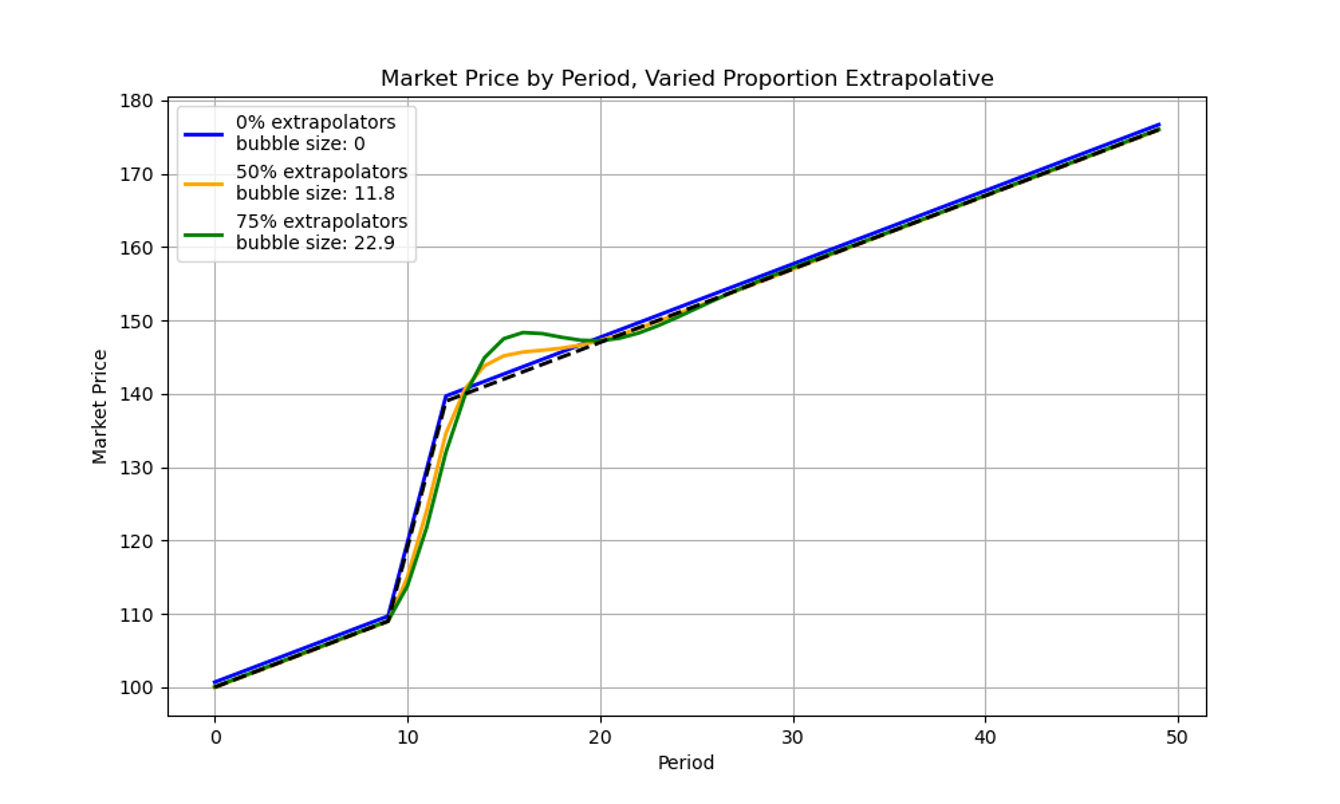
\includegraphics[width=0.8\linewidth]{images/bubbles1.png}
    \label{fig:enter-label}
\end{figure}
Note that when there are no extrapolators in the market, denoted by the blue line, the jump in fundamental value does not trigger a bubble. This scenario represents the predictions of standard economic theory, in which people behave rationally and bubbles therefore do not form. Introduction of extrapolators causes the jump in fundamental value to trigger a bubble, and higher proportions of extrapolators cause larger bubbles.

I next fix the proportion of extrapolators at 75\% and investigate the effect of allowing the rational agents to know about the existence of the extrapolative ones. This is shown in the graph below, with the yellow line representing the price movemment when the rational agents do not know about the extrapolators, and the green line representing the price movement when they do.

\begin{figure}[H]
    \centering
    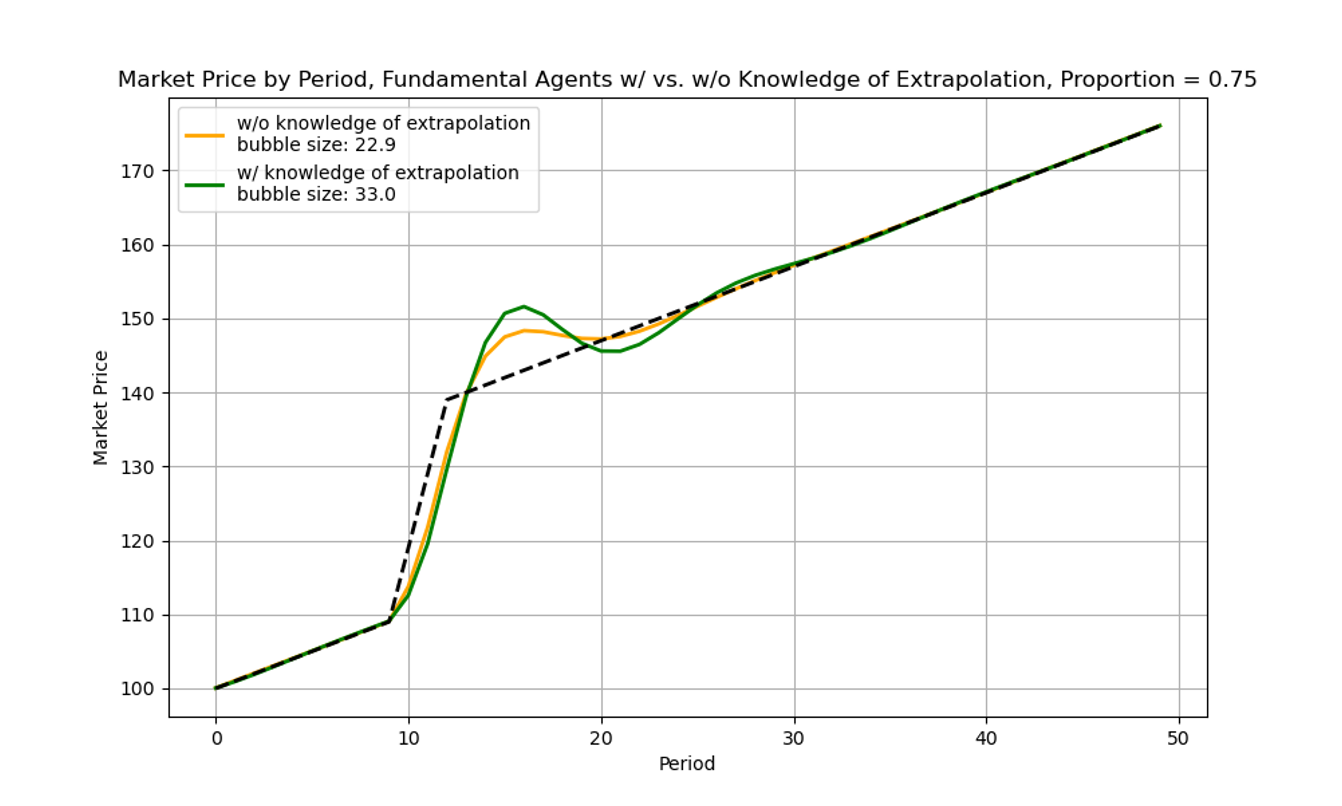
\includegraphics[width=0.8\linewidth]{images/bubbles2.png}
    \label{fig:enter-label}
\end{figure}
Predictably, I find that allowing rational agents to know about extrapolative ones increases the size of the bubble, in this case by about 44\%. This result makes sense because if rational agents know that there are extrapolative agents, they know that mispricings will not be immediately corrected. They therefore have an incentive not to sell immediately when the bubble begins, but rather to hold with the expectation it will continue to grow. This pushes up price. 

I then investigate what impact the proportion of extrapolative agents has on the magnitude of the impact that rational agents knowing about extrapolative ones has on bubble size. The figure below plots bubble size against the proportion of extrapolative agents. In green are the values when rational agents know about extrapolators, and in yellow are the values when they don't.

\begin{figure}[H]
    \centering
    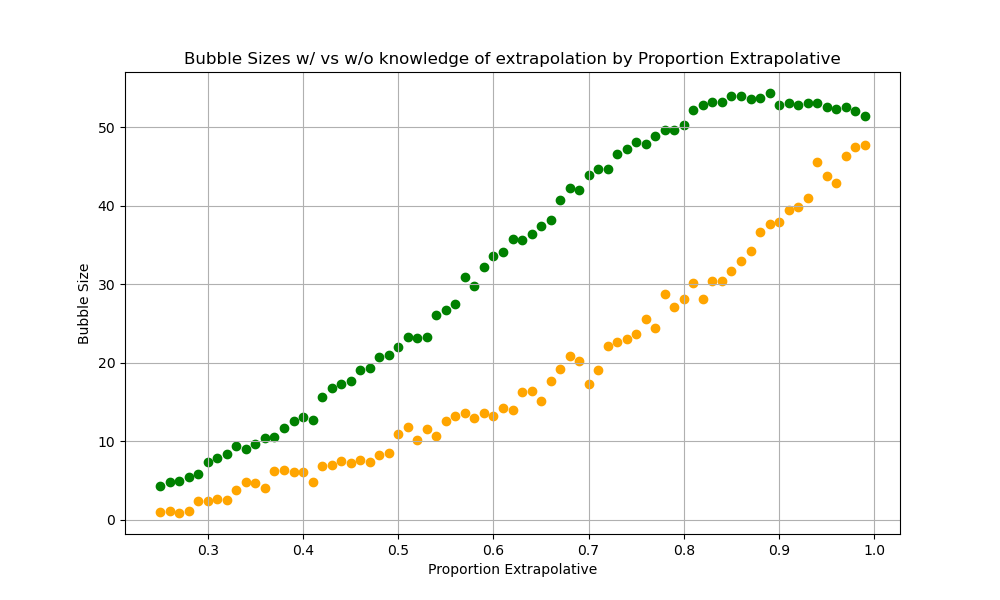
\includegraphics[width=0.8\linewidth]{images/bubbles3.png}
    \label{fig:enter-label}
\end{figure}

I find that bubbles are larger when rational agents have knowledge of extrapolation at every proportion of extrapolators, but that the magnitude of that difference varies. To get a better sense of how much in relative terms, I create the graph shown below. It plots the ratio of bubble sizes, where a value of 1 means that there is no difference between bubble size when rational agents have knowledge of extrapolation and when they don't, and a vale of 0 means there is infinite difference. 

\begin{figure}[H]
    \centering
    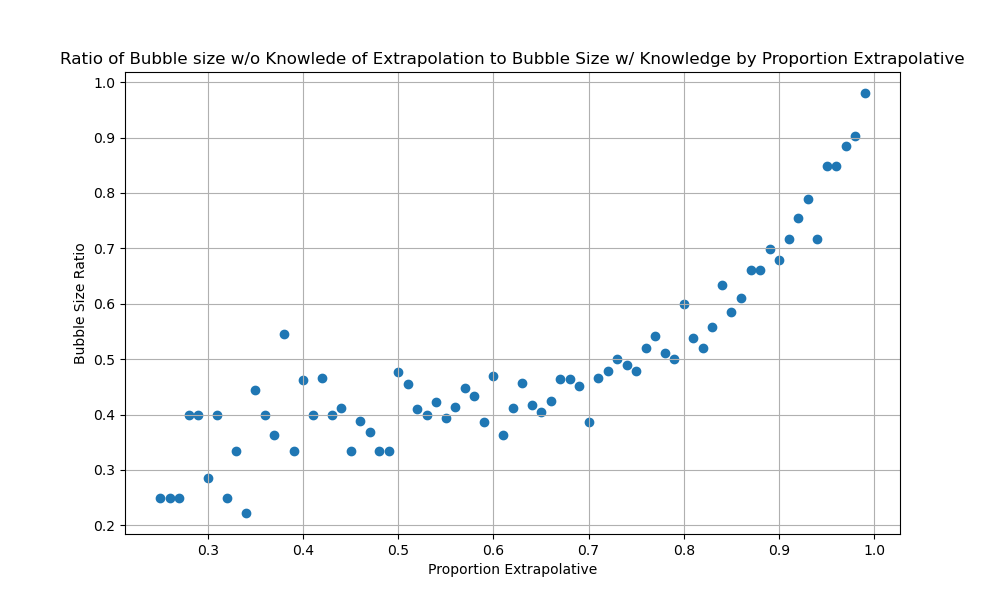
\includegraphics[width=0.8\linewidth]{images/bubbles4.png}
    \label{fig:enter-label}
\end{figure}

I find that as the proportion of extrapolative agents decreases, the bubble size ratio decreases at a decreasing rate. This means that if most market participants have extrapolative beliefs, rational participants taking that into account does not lead to a large increase in bubble size. If few market participants have extrapolative beliefs, the rational ones taking that into account will lead to much larger bubbles than otherwise. 

This work expands on that of Barberis et. al\cite{BarberisEtAl} by introducing rational agent's knowledge of extrapolative ones into their existing model of bubble formation. While my results provide an estimate of the effects of doing so on bubble size, they have significant limitations. First, the model assumes all rational agents either account for or don't account for extrapolation. This is unrealistic as in the real world some will and some won't. A better question to ask might therefore be given the mean estimate of the proportion of people who are extrapolative, what proportion of rational people must be accounting for this to create a bubble of a given size. However, this question is outside the scope of my work. Second, my model does not account for the radical variation in market-moving ability across various investors, and the extent to which higher market-moving ability, i.e. institutional investors, is correlated with more sophisticated, i.e. rational, trading strategies. 

\subsection{Underinvestment}
The graph below shows the paths of consumption and wealth over the lifetime for agents who are present biased and for those who aren't. Wealth is denoted by a solid line and consumption by a dashed one. The orange lines are the values for a present biased agent, and the blue ones are the values for one who isn't. 
\begin{figure}[H]
    \centering
    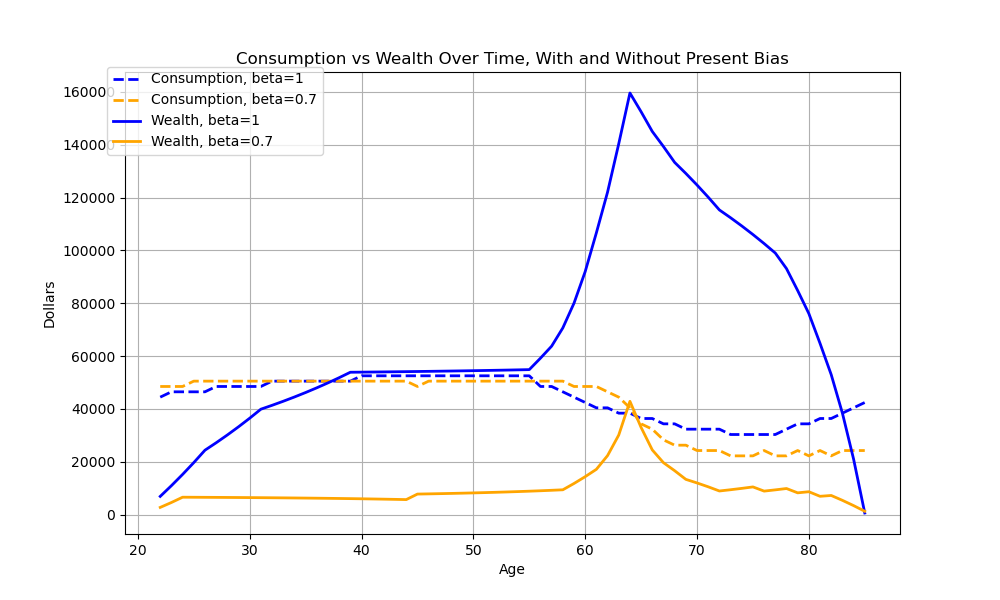
\includegraphics[width=0.8\linewidth]{images/underinvestment4.png}
    \label{fig:enter-label}
\end{figure}
The first thing to notice is that the wealth for both agents grows over the course of their working lives and shrinks over the course of their retirement. This is the result of positive savings rates. The wealth of the agent who is not present biased is larger than that of the agent who is, both on average and at the maximum. This is because the agent who is not present biased has the self control to save slightly more than the one who is, meaning they are able to accumulate savings which compound over time. The consumption for both agents falls during retirement. However, the consumption for the non-present-biased agents falls by less because they have more wealth from which they can draw.

Of the three simulations, this is the one from which the least can be gained. The assumptions made are more unrealistic than in the others, and the decision-making mechanism is less sophisticated than other similar work. Unlike the other two, there is nothing novel that this simulation does, even if marginally so. All I can claim about the usefulness of the simulation is that it was interesting to create. Still, I think it is worth including. It helps to widen the collection of psychology concepts that can be added to models to make them more accurate, and therefore contributes to my project's goal of making a general argument for the merit of doing so. 

\section{Ethical Considerations}
Because my project is not user-facing, there are no ethical considerations related to accessibility. There is minimal data used, meaning questions of data selection or privacy are irrelevant. My project is not plausibly monetizable, meaning there are no issues of competing incentives between revenue and other considerations. Instead, my project is a research project, and its ethical considerations are limited to the ways its results could influence policy-making. While I do not realistically expect the work of this project to in any way influence any policy decisions, the more general discussion of how policy-makers should account for behavioral economic research is still an interesting one. I have already discussed specific limitations of each of my simulation in the previous section. This section will focus more on general considerations than ones specific to any research topic.

\subsection{Potential of Behavioral Economic Research to Improve Welfare}
The ways that behavioral economic research could improve welfare, defined as aggregate measures of utility within a society, are straightforward. Economic models are already used in the formulation of various public policies by government agencies. If those models are flawed, their recommendations will be suboptimal. Improving the models by introducing concepts from behavioral economics would improve welfare, assuming that welfare maximization is the sole goal of the policy-maker. As an example, Lehr (2024) finds that models of the optimal structure of the United State's social security system generate significantly different results when accounting for loss aversion.\cite{lehrLossAversion} Assuming that loss aversion is a true aspect of human nature, welfare would be improved if policy-makers adopted models of optimal social security structure which included it.  

\subsection{Potential of Behavioral Economic Research to Worsen Welfare}
Behavioral economic research has the potential to worsen welfare either if policy-makers who utilize it have goals other than welfare maximization, or if the research is flawed to the extent that application of its results worsens the recommendations of models from a welfare-maximization perspective. An example of behavioral economic research being used to worsen welfare is if it's insights are used by businesses for the purpose of increasing profits rather than increasing welfare. Trevisan (2015) explores numerous manifestations of this.\cite{Trevisan} Consumer behavior as a result of businesses implementing these strategies may result in outcomes they are unhappy with relative to their decisions prior, worsening welfare. Even when used by benevolent policy-makers, research that is sufficiently flawed could lead to worse outcomes. That is, even if the effect being studied is real, if its estimation is wrong enough the magnitude of the resulting correction to policy could lead to worse outcomes than ignoring the effect completely.

\subsection{Implications}
The implication of these potential welfare effects for researchers is to be as transparent as possible about the limitations of their research so that it is less likely to be used without appropriate caution by policy-makers. For policy-makers, the implication is firstly to pay attention to the research, as it may reveal opportunities for improved policy. As is true in all contexts, they should ensure they understand the research's methods and assumptions sufficiently to not over-read its results. Additionally, an investigation of the behavioral economics literature may reveal opportunities for effective consumer protection measures. 

\printbibliography
\appendix
\section{Replication Instructions}
Replicating my project is very straightforward. First, clone the following repository: \url{https://github.com/owilkins2/Comps_Final} 

Download the dependencies listed in the requirements.txt file in the 'Code' folder. From there you can run any of the simulations, which are each a single python file, and experiment with whatever changes you would like. I ran the simulations in the command line and edited them in Visual Studio, although you can use whatever system you choose. 


\section{Code Architecture Overview}
Someone who wanted to extend my project would likely do so in one of three ways:
\begin{enumerate}
    \item Change the chosen parameters
    \item Change the decision-making logic of the agent(s)
    \item Change the way data is visualized
\end{enumerate}
Each simulation is a single file. I will describe where in the file someone who wanted to do one of the above should start looking. 
\begin{enumerate}
    \item Most parameters are listed either at the top of the file or at the bottom as part of the calls to the various functions. However, there are some instances where the parameters are included in the functions themselves. These are usually cases where the parameter in question is a coefficient for which there is a well-established literature estimating it (e.g. the coefficient of risk aversion). Any value having to do with subjective decisions about the running of the simulation (e.g. how many periods it lasts for) should be at either the top or bottom of the file. 
    \item The agent decision-making logic is contained within the various functions in the file. Generally speaking, the functions at the top of the file deal with the explicit decision-making process, where those further down have to do with the administration of the simulation. The function names should be useful in determining their purpose. 
    \item The visualizations are created at the bottom of the file, after the various functions have been called to run the simulation and return results. If you want to change the way that the existing data is visualized, you can restrict your edits to the sections after the results have been returned. If you want new data to be collected as the simulation runs, that will require editing of the various functions which administer the running of the simulation.
\end{enumerate}
\end{document}
    